\tituloProblema{1}{Problema}
Vocês naufragaram em uma ilha deserta e o prazo do projeto de programação está terminando.
Vocês codificaram o programa em uma linguagem de programação de alto nível utilizando computadores
portáteis, mas não sabem como transmiti-lo.
No último momento um barco de pesca salva vocês, que percebem que existe um telégrafo no barco, então levantam três perguntas:
\begin{enumerate}
    \item Podemos telegrafar o código do programa por alfabeto \textit{Morse}?
    \item E o programa executável, é possível transmitirmos utilizando o alfabeto \textit{Morse}?
    \item Quais os tipos de linguagens que podemos geralmente codificar utilizando o alfabeto \textit{Morse}?
\end{enumerate}

Para trazer um pouco de dificuldade para quem eventualmente interceptar as mensagens transmitidas
utilizando o telégrafo, vocês decidem que dentro das possibilidades de transmissão do código do programa
e do executável irão incluir uma espécie de criptografia simplificada utilizando as operações
em linguagens formais.

\begin{figure}[!htb]
\centering
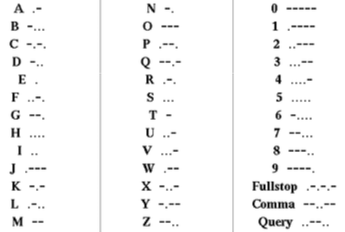
\includegraphics[scale=0.5]{apendice/problemas/problema1a/fig2.png}
\caption{Alfabeto \textit{Morse}}
\label{fig2}
\end{figure}

\tituloProblema{2}{Produto}
Um relatório no modelo de artigos da SBC com uma discussão detalhada sobre as três perguntas levantadas
e sobre a criptografia simplificada.
\tituloProblema{3}{Cronograma}

1 sessão tutorial e 1 aula expositiva.

\tituloProblema{4}{Recursos para aprendizagem}

\noindent
RAMOS, M. V. M.; JOSÉ NETO, J.; VEGA, I. S. \textbf{Linguagens Formais: Teoria, Modelagem e Implementação}. Editora Bookman, 2009.\\

\noindent
MENEZES, Paulo Blauth. \textbf{Linguagens formais e autômatos}. 6. ed. Bookman, 2011.\\

\tituloProblema{$*$}{Referências}

Este problema é baseado no texto da Wilhelmiina Hamalainen\footnote{\url{https://www.researchgate.net/profile/Wilhelmiina_Haemaelaeinen}}.
